\documentclass[a4paper]{article}

%% Language and font encodings
\usepackage[english]{babel}
\usepackage[utf8x]{inputenc}
\usepackage[T1]{fontenc}

\usepackage{multicol}

%% Sets page size and margins
\usepackage[a4paper,top=3cm,bottom=2cm,left=3cm,right=3cm,marginparwidth=1.75cm]{geometry}

%% Useful packages
\usepackage{amsmath}
\usepackage{graphicx}
\usepackage[colorinlistoftodos]{todonotes}
\usepackage[colorlinks=true, allcolors=blue]{hyperref}

\title{CS170: Assignment 1 Write Up}
\author{Audrey Der, 861221280}

\begin{document}
\maketitle

%\begin{abstract}
%Your abstract.
%\end{abstract}

\section{Introduction}

This assignment is the first project in Dr. Eamonn Keogh's Introduction to AI
course at the University of California, Riveside during the quarter of Fall
2017. The following write up is to detail my findings through the course of
project completion. \\ \\ It explores Uniform Cost Search, and the Misplaced Tile and
Manhattan Distance heursitics applied to A*. My lanugage of choice was Python
(version 3), and the full code for the project is included.

\section{Comparison of Algorithms}
The three algorithms implemented are as follows: Uniform Cost Search, A* using
the Misplaced Tile heuristic, and A* using the Manhattan Distance heuristic.

\subsection{Uniform Cost Search}
As noted in the initial assignment prompt, \textbf{Uniform Cost Search} is simply A* with
h(n) hardcoded to 0, and it will only expand the cheapest node, whose cost is in
g(n). In the case of this assignment, there are no weights to the expansions,
and each expanded node will have a cost of 1.

\subsection{The Misplaced Tile Heuristic}
The second algorithm implemented is A* with the \textbf{Misplaced Tile Heuristic}. The
heuristic looks to the number of ``misplaced'' tiles in a puzzle. For example:
\begin{verbatim}
A puzzle:
[[1, 2, 4],
 [3, 0, 6],
 [7, 8, 5]]
\end{verbatim}

...and it's goal state:
\begin{verbatim}
goal state:
[[1, 2, 3],
 [4, 5, 6],
 [7, 8, 0]]
\end{verbatim}

Not counting 0 (the placeholder for the blank/missing tile), g(n) is set to the
 number of tiles not in their current goal state position are counted; in this
 example, g(n) = 3. This assigns a number, where lower is better, to node
 expansion based on how many misplaced tiles there are after any given position
 change of the space. When applied to the n-puzzle, queue will expand the node
 with the cheapest cost, rather than expanding each of the child nodes as
 Uniform Cost Search would.

 \subsection{The Manhattan Distance Heuristic}
 The \textbf{Manhattan Distance Heuristic} is similar to the Misplaced Tile
 Heuristic such that it considers the cost of future expansions and looks at
 misplaced tiles, but has a different rationale to it. The heuristic considers
 all of the misplaced tiles \textit{and} the number of tiles away from its goal
 state position would be. The resulting g(n) is the sum of all the cost of all
 misplaced tile distances. Using the example above:
\begin{verbatim}
A puzzle:
[[1, 2, 4],
 [3, 0, 6],
 [7, 8, 5]]

goal state:
[[1, 2, 3],
 [4, 5, 6],
 [7, 8, 0]]

\end{verbatim}
Not counting the position of 0, it can be seen that tiles 4, 3, and 5 are out of
place. Based on their positions in the puzzle and their goal state positions,
g(n) = 8. 
\subsection{Comparison of Algorithms on Sample Puzzles}
There were six puzzles of varying difficulty given to implement. The easiest
of the six is a trivial puzzle (the puzzle being the goal state) and the hardest puzzle
is impossible to solve (the goal state, but the position of tiles 7 and 8
swapped). The puzzle configurations themselves can be seen in nPuzzle.py.
See Figure 1 and Figure 2 for a visual representation of the number of nodes
expanded and the maximum queue size, respectively. \\ \\ It was found that the
difference between the three algorithms was relatively negligible when given
easier puzzles, but the heuristics (and how good the heuristic was) made a
significant difference in the space complexity when solving more difficult but
still solvable puzzles. 

\begin{figure}
  \centering
  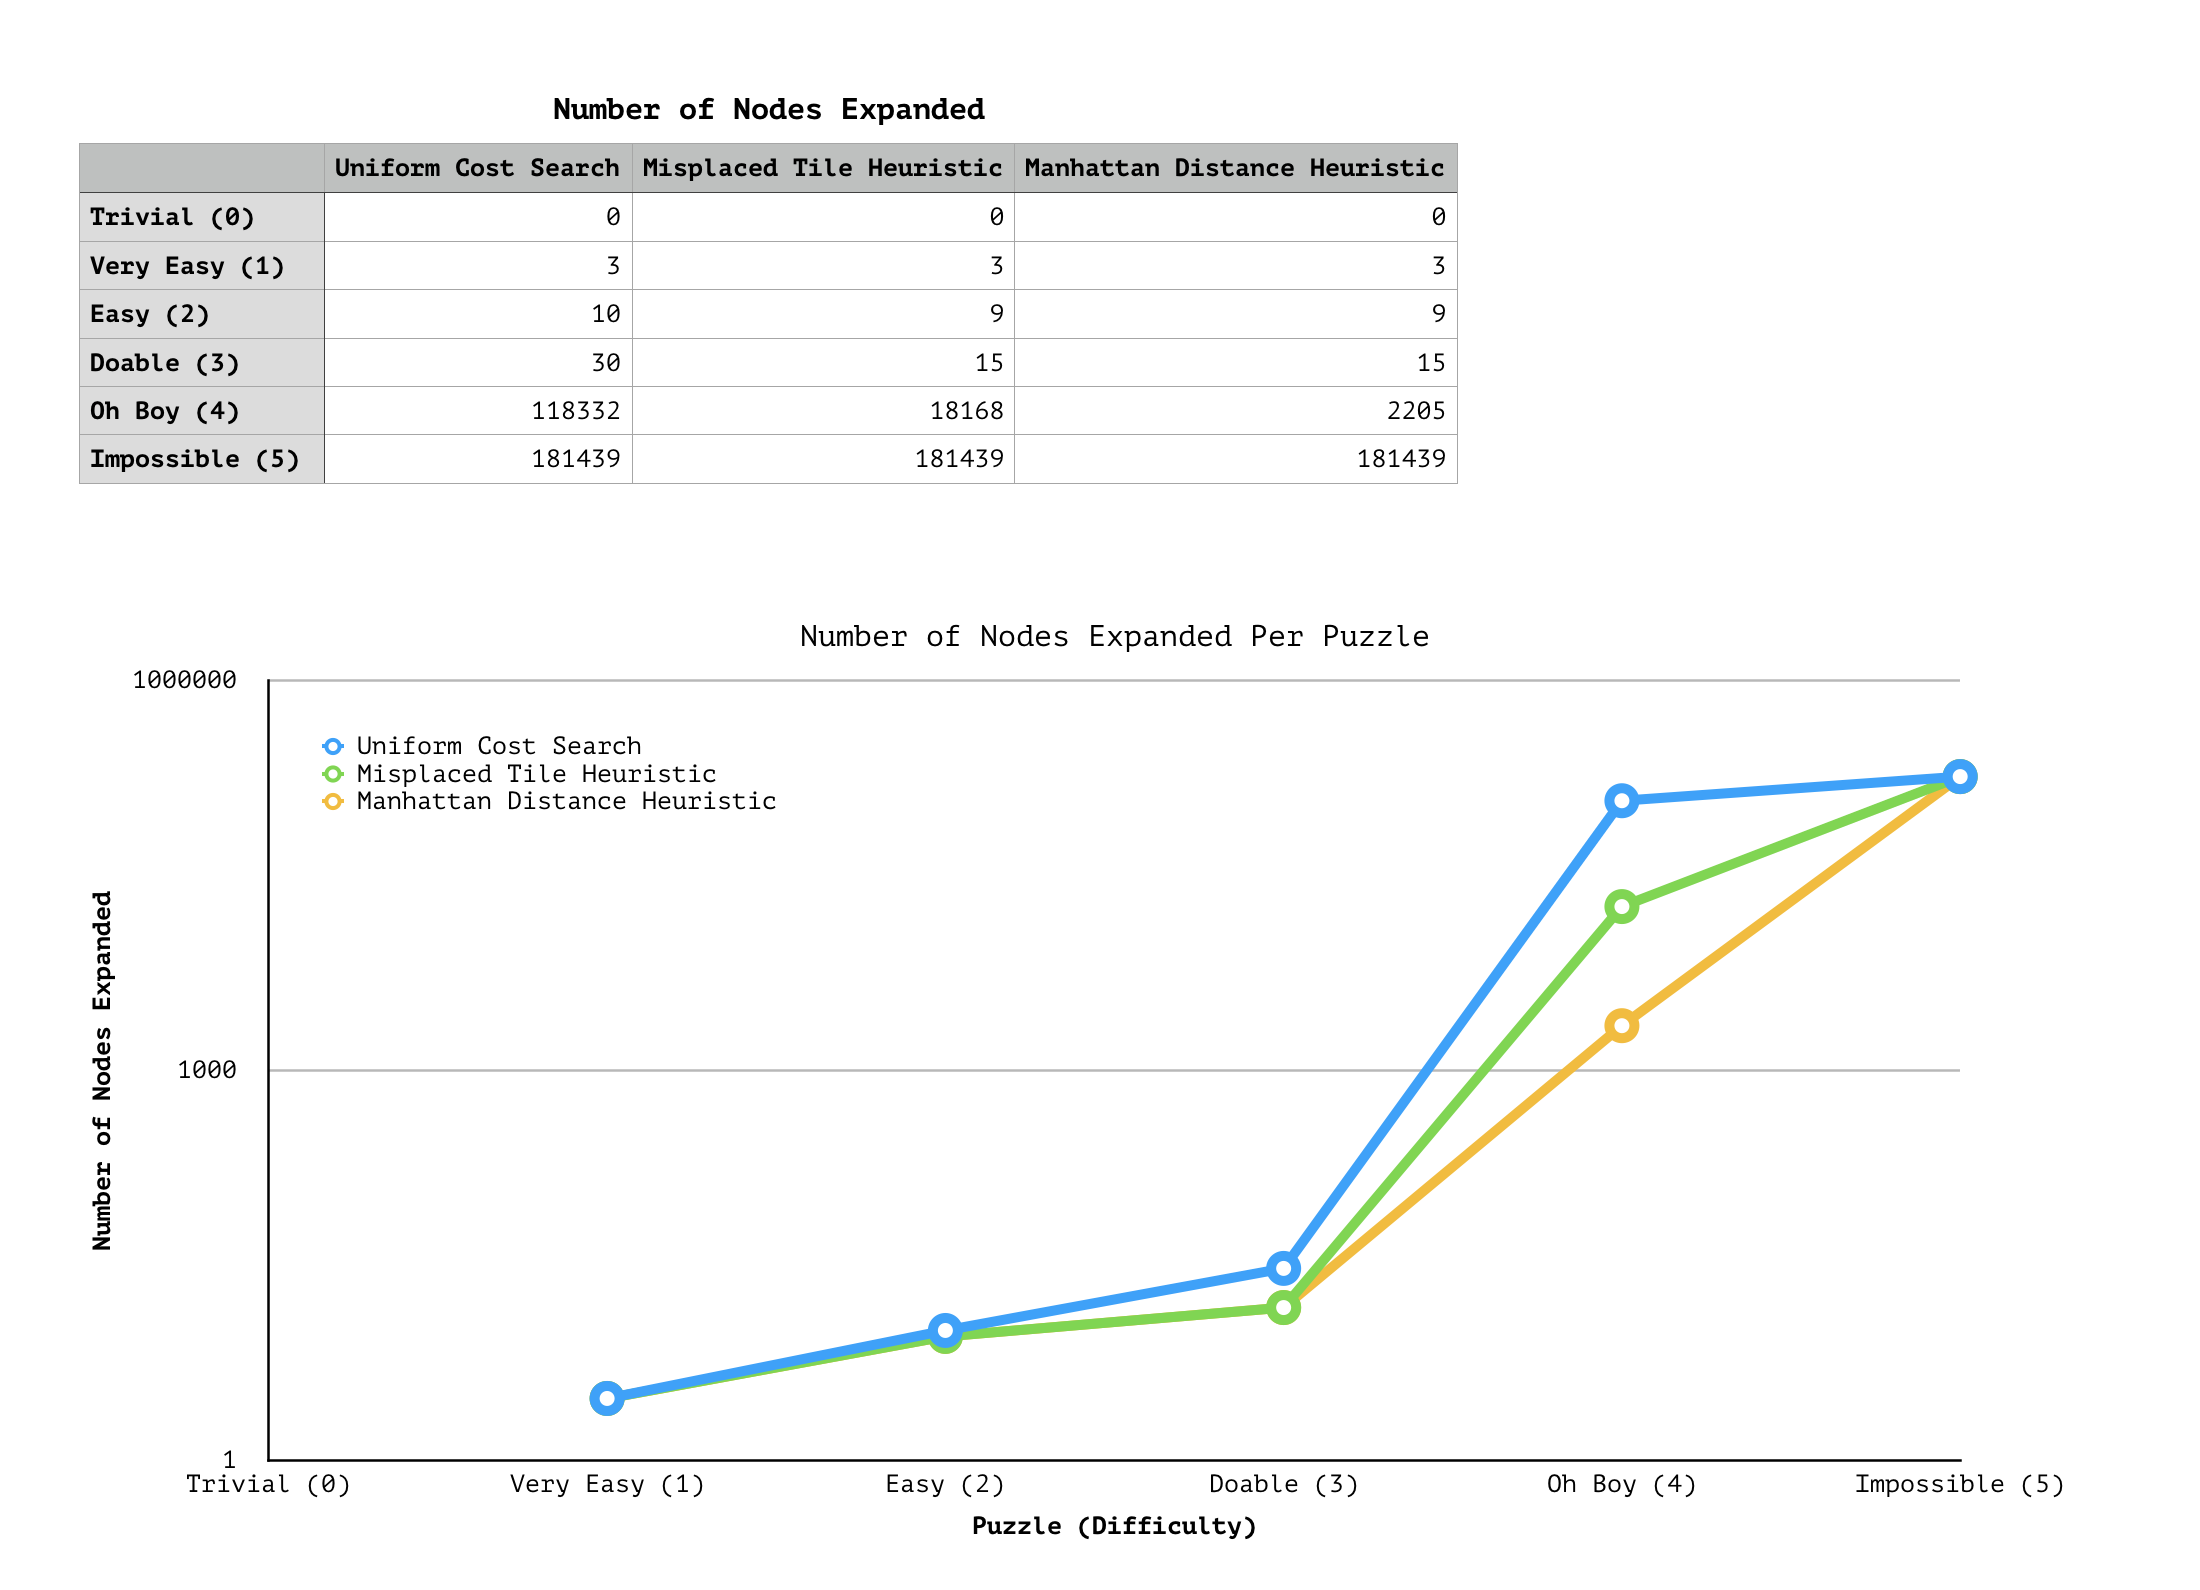
\includegraphics[width=\paperwidth, angle=90]{Number Nodes Expanded.png}
  \label{Figure 1}
\end{figure}

\begin{figure}
  \centering
  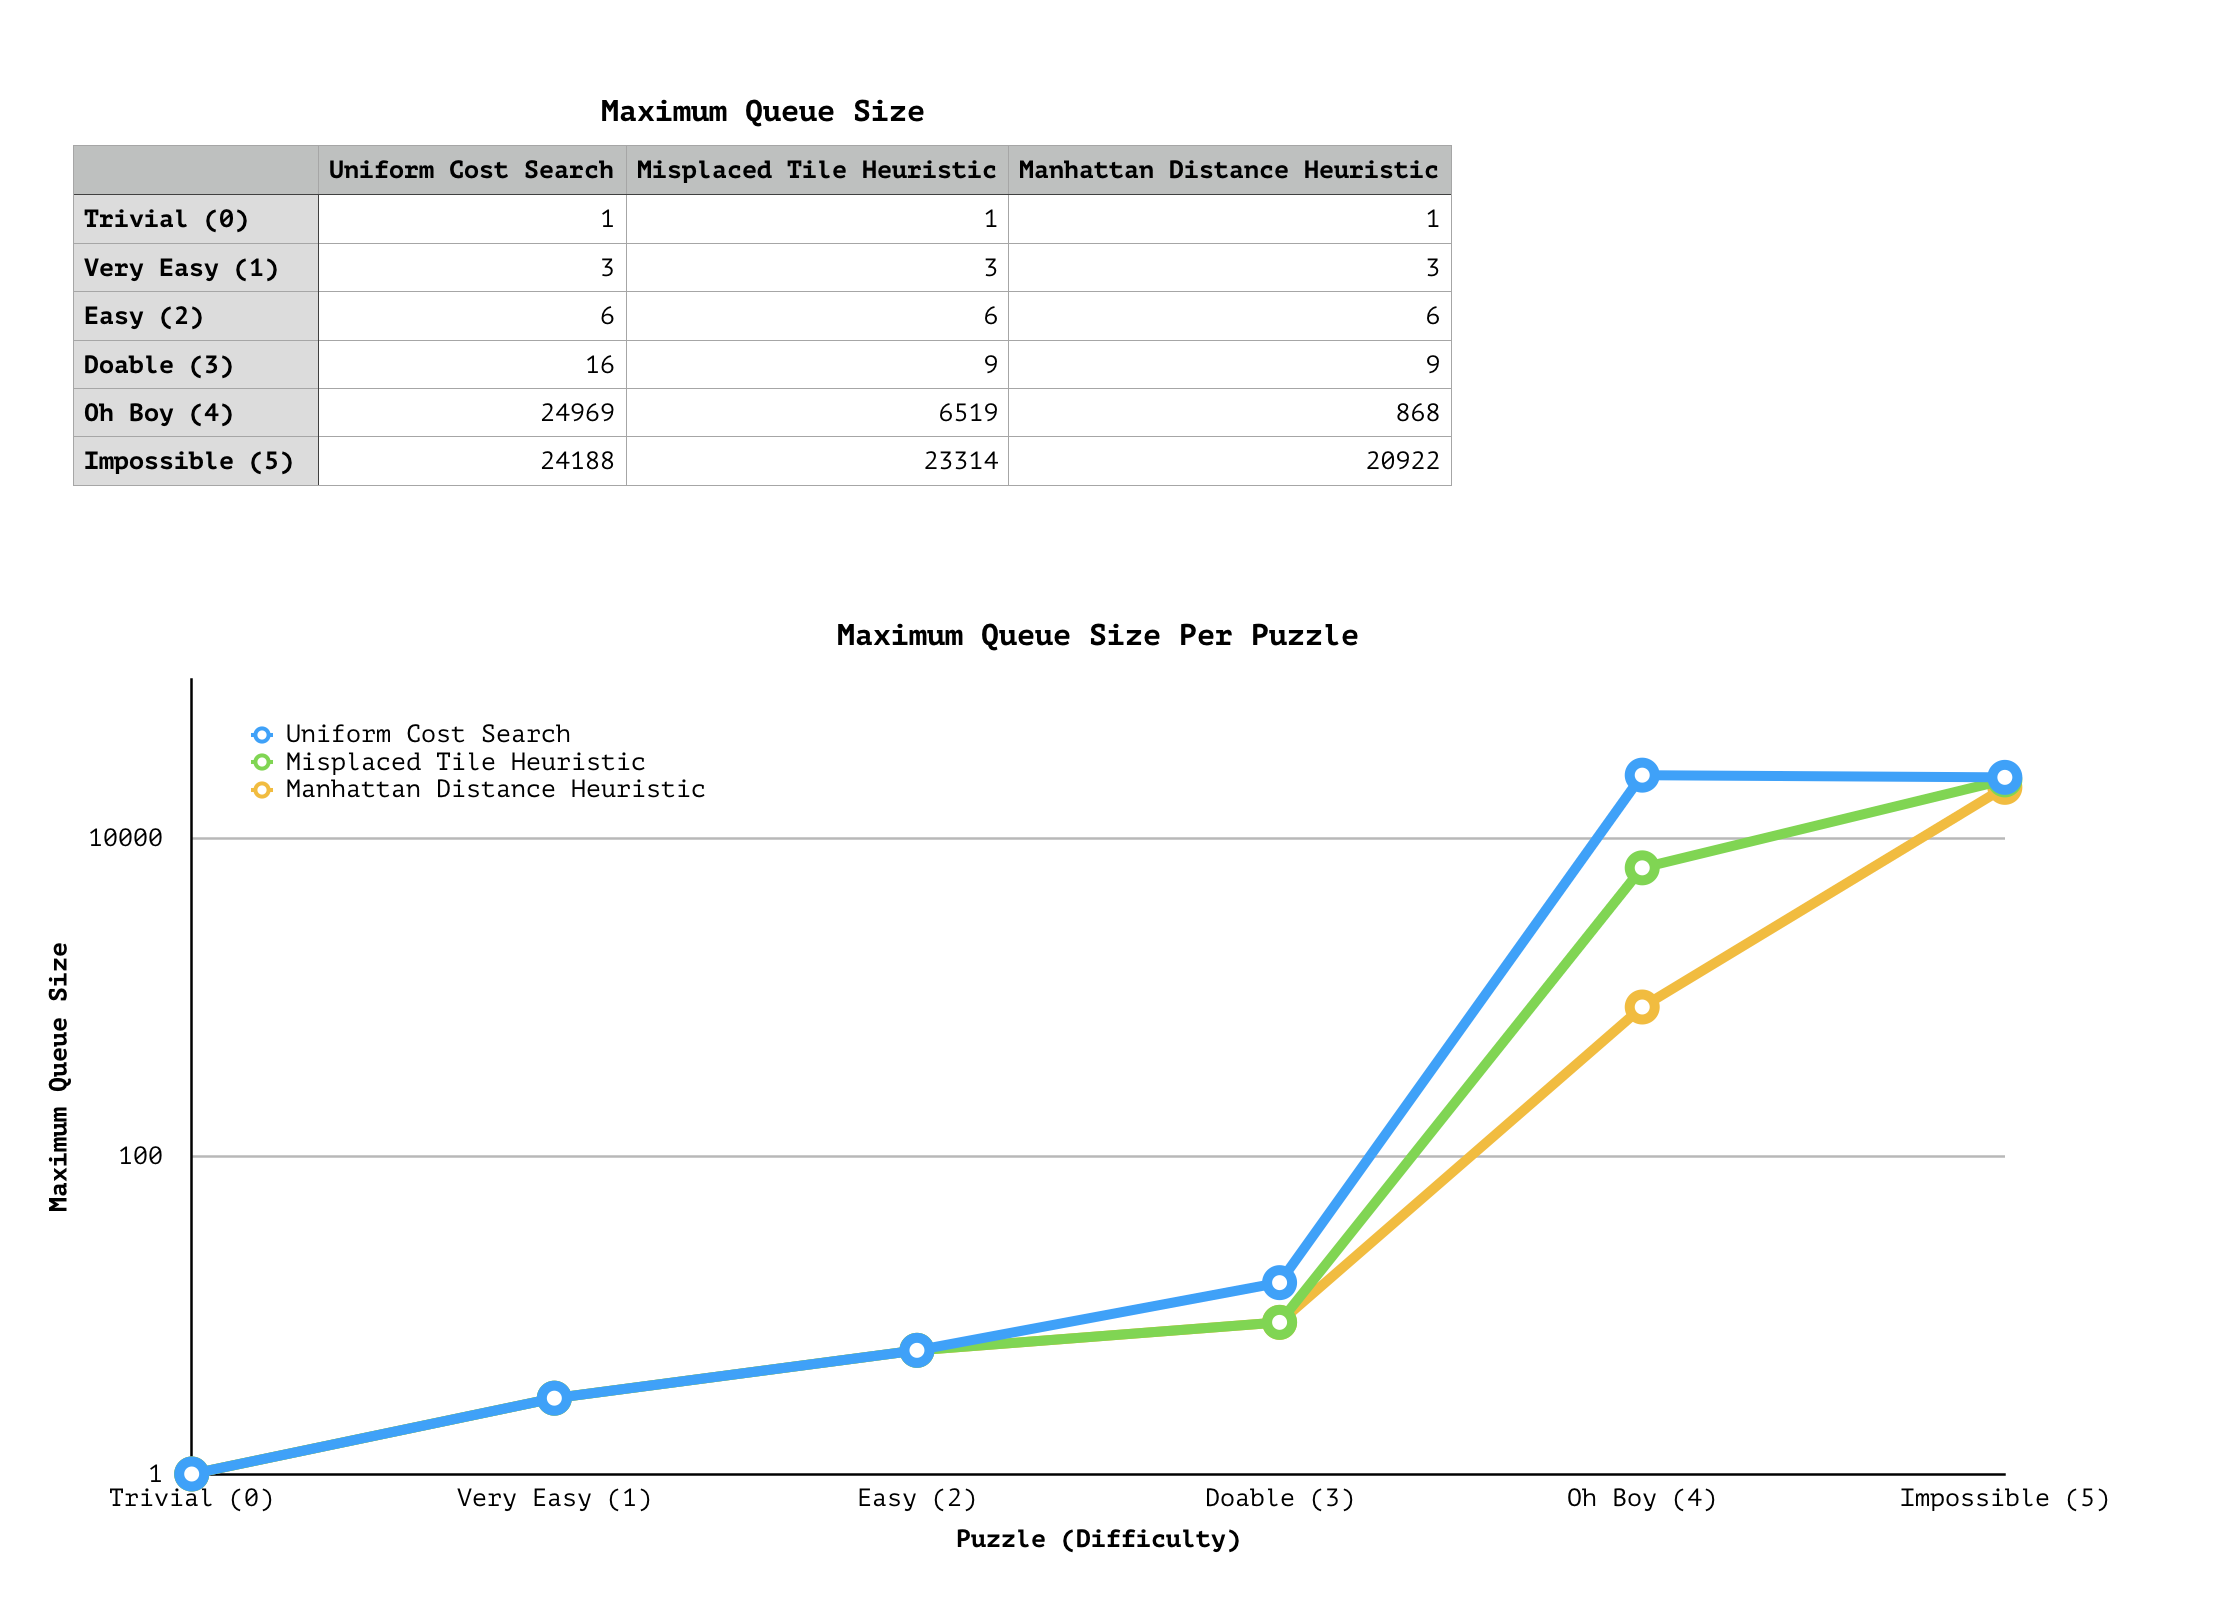
\includegraphics[width=\paperwidth, angle=90]{Maximum Queue Size.png}
  \label{Figure 2}
\end{figure}

\section{Mathematic Verification} %some proof that the actual space complexity is
                                %consistent with the theory space complexity
\section{Example Traceback}
This section is the output (in three columns) from the assignment on puzzle 3,
Doable, for Uniform Cost Search and the Misplaced Tile heuristic. \\

\begin{multicols}{3}
  [
  Algorithm: Uniform Cost Search, Puzzle: Doable
  Nodes expanded: 30, Max queue size: 16
  ]
\begin{verbatim}

[4, 1, 2]
[5, 3, 0]
[7, 8, 6]

[4, 0, 2]
[5, 1, 3]
[7, 8, 6]

[4, 1, 2]
[5, 8, 3]
[7, 0, 6]

[1, 5, 2]
[4, 3, 0]
[7, 8, 6]

[1, 5, 2]
[4, 8, 3]
[7, 0, 6]

[1, 5, 2]
[0, 4, 3]
[7, 8, 6]

[4, 1, 2]
[7, 5, 3]
[8, 0, 6]

[1, 2, 3]
[4, 5, 0]
[7, 8, 6]

[1, 5, 2]
[4, 0, 3]
[7, 8, 6]

[4, 1, 2]
[7, 5, 3]
[0, 8, 6]

[4, 1, 2]
[5, 0, 3]
[7, 8, 6]

[1, 2, 0]
[4, 5, 3]
[7, 8, 6]

[4, 1, 2]
[0, 5, 3]
[7, 8, 6]

[1, 0, 2]
[4, 5, 3]
[7, 8, 6]

[0, 1, 2]
[4, 5, 3]
[7, 8, 6]

\end{verbatim}
\end{multicols}
\begin{multicols} {3}
  [
  Algorithm: Misplaced Tile Heuristic, Puzzle: Doable
  Nodes expanded: 15, Max queue size: 9
  ]
\begin{verbatim}

[1, 2, 3]
[4, 0, 5]
[7, 8, 6]

[1, 2, 3]
[4, 5, 0]
[7, 8, 6]

[1, 5, 2]
[4, 0, 3]
[7, 8, 6]

[1, 2, 0]
[4, 5, 3]
[7, 8, 6]

[4, 1, 2]
[0, 5, 3]
[7, 8, 6]

[1, 0, 2]
[4, 5, 3]
[7, 8, 6]

[0, 1, 2]
[4, 5, 3]
[7, 8, 6]

\end{verbatim}
\end{multicols}

%\section{Closing Thoughts}
% The most interesting thing to me was realizing that as impractical Breadth First Search and
% Depth First Search are in the context of real world problems, they are still the
% heart of some practical, feasible algorithms used for such real world problems.

\end{document}